
\begin{center}
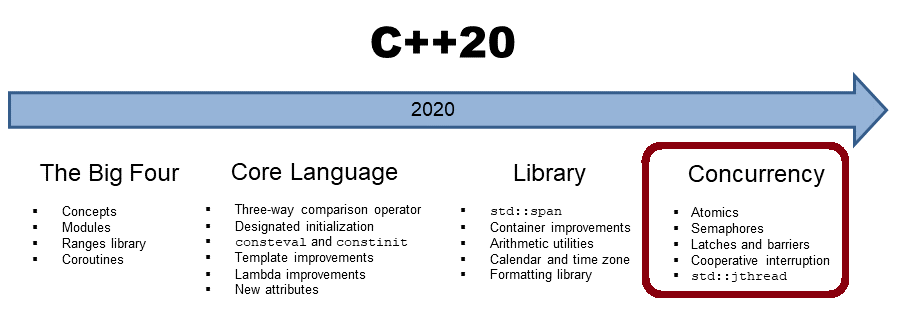
\includegraphics[width=1.0\textwidth]{content/2/chapter3/images/7.png}\\
\end{center}

\subsubsubsection{3.4.1\hspace{0.2cm}原子变量和操作}

类模板std::atomic\_ref对引用的非原子对象应用原子操作。因此,可以对其进行并发的读写,不会出现数据竞争。引用对象的生存期必须超过std::atomic\_ref的生存期。使用std::atomic\_ref访问引用对象的子对象时,并不是线程安全的。

根据\href{https://en.cppreference.com/w/cpp/atomic/atomic}{std::atomic},std::atomic\_ref可以特化,并支持内置数据类型的特化。

\begin{lstlisting}[style=styleCXX]
struct Counter {
	int a;
	int b;
};

Counter counter;

std::atomic_ref<Counter> cnt(counter);
\end{lstlisting}

C++20中,有两个原子智能指针,是std::atomic的偏特化,分别是std::atomic<std::shared\_ptr<T>>和std::atomic<std::weak\_ptr<T>>。这两个原子智能指针不仅保证控制块(如\href{https://en.cppreference.com/w/cpp/memory/shared_ptr}{std::shared\_ptr})是线程安全的,而且还保证关联对象是线程安全的。

std::atomic有更多的扩展,C++20为原子浮点类型提供了特化。当需要并发递增的浮点类型时,就可以直接使用了。

类型\href{https://en.cppreference.com/w/cpp/atomic/atomic_flag}{std::atomic\_flag}是一种原子布尔值,有一个清除和设置状态。简单起见,这里将clear状态称为false,set状态为true。clear()成员函数允许将其值设置为false。使用test\_and\_set()成员函数,可以将值设置为true,并获得之前的值。没有成员函数可以获取当前值。这将在C++20中改变,因为std::atomic\_flag添加了一个test()方法。

此外,std::atomic\_flag可以通过成员函数notify\_one()、notify\_all()和wait()用于线程同步。C++20中,通知和等待在std::atomic和std::atomic\_ref的所有偏特化和全特化上都可用。特化可用于bool、整型、浮点数和指针。

\subsubsubsection{3.4.2\hspace{0.2cm}信号量}

信号量是一种同步机制,用于控制对共享资源的并发访问。计数信号量,例如C++20中添加的计数信号量,是一种特殊的信号量,其初始计数器大于零。计数器在构造函数中初始化。获取信号量会减少计数器,释放信号量则会增加计数器。若线程试图在计数器为零时获取信号量,线程将阻塞,直到另一个线程通过释放信号量来增加计数器。


\subsubsubsection{3.4.3\hspace{0.2cm}门闩和栅栏}

门闩和栅栏是线程的同步机制,可以使一些线程阻塞,直到计数器为零。这两种同步线程的机制有什么不同?std::latch只能使用一次,但std::barrier可以使用多次。std::latch在多线程管理一个任务时很有用,barrier对于管理多线程的重复任务。此外,std::barrier可以在每次迭代中调整计数器。

以下是基于提案\href{http://www.open-std.org/jtc1/sc22/wg21/docs/papers/2014/n4204.html}{N4204}的代码片段。我修正了一些错别字,重新进行了格式化。

\hspace*{\fill} \\ %插入空行
\noindent
\textbf{使用std::latch进行线程同步}
\begin{lstlisting}[style=styleCXX]
void DoWork(threadpool* pool) {

	std::latch completion_latch(NTASKS);
	for (int i = 0; i < NTASKS; ++i) {
		pool->add_task([&] {
			// perform work
			...
			completion_latch.count_down();
		});
	}
	// Block until work is done
	completion_latch.wait();
}
\end{lstlisting}

std::latch的completion\_latch的计数器设置为NTASKS(第3行)。线程池执行NTASKS作业(第4-10行)。任务结束时,计数器递减(第8行)。运行DoWork函数的线程在第12行阻塞,直到所有任务都完成。

\subsubsubsection{3.4.4\hspace{0.2cm}中断协程}

std::stop\_token可以中断std::jthread。

\hspace*{\fill} \\ %插入空行
\noindent
\textbf{中断std::jthread}
\begin{lstlisting}[style=styleCXX]
int main() {
	
	std::cout << '\n';
	
	std::jthread nonInterruptible([]{
		int counter{0};
		while (counter < 10){
			std::this_thread::sleep_for(0.2s);
			std::cerr << "nonInterruptible: " << counter << '\n';
			++counter;
		}
	});
	
	std::jthread interruptible([](std::stop_token stoken){
	int counter{0};
	while (counter < 10){
		std::this_thread::sleep_for(0.2s);
			if (stoken.stop_requested()) return;
			std::cerr << "interruptible: " << counter << '\n';
			++counter;
		}
	});
	
	std::this_thread::sleep_for(1s);
	
	std::cerr << '\n';
	std::cerr << "Main thread interrupts both jthreads" << std:: endl;
	nonInterruptible.request_stop();
	interruptible.request_stop();
	
	std::cout << '\n';
	
}
\end{lstlisting}

主程序启动两个线程,nonInterruptible和interruptible(第5行和第14行)。只有线程可中断得到std::stop\_token,在第18行中使用它来检查是否中断。在中断的情况下,Lambda立即返回。调用interruptible.request\_stop()会触发线程的取消,并且nonInterruptible.request\_stop()没有任何效果。

\begin{center}
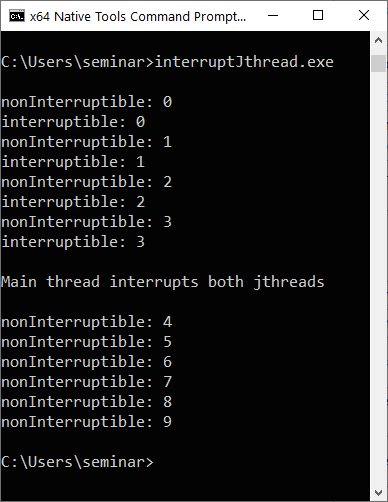
\includegraphics[width=0.6\textwidth]{content/2/chapter3/images/8.png}\\
协程的中断
\end{center}

\subsubsubsection{3.4.5\hspace{0.2cm}std::jthread}

std::jthread代表连接线程。std::jthread通过自动加入已启动的线程扩展\href{https://en.cppreference.com/w/cpp/thread/thread}{std::thread}。std::jthread也可以被中断。

因为std::thread的非直观行为,所以std::jthread添加到C++20标准中。若std::thread仍可汇入,\href{https://en.cppreference.com/w/cpp/error/terminate}{std::terminate}将在其析构函数中进行汇入。若既没有调用thr.join(),也没有调用thr.detach(),那么线程thr是可汇入的。

\hspace*{\fill} \\ %插入空行
\noindent
\textbf{线程thr仍然是可汇入的}
\begin{lstlisting}[style=styleCXX]
int main() {
	
	std::cout << '\n';
	
	std::cout << std::boolalpha;
	std::thread thr{[]{ std::cout << "Joinable std::thread" << '\n'; }};
	std::cout << "thr.joinable(): " << thr.joinable() << '\n';
	
	std::cout << '\n';
}
\end{lstlisting}

\begin{center}
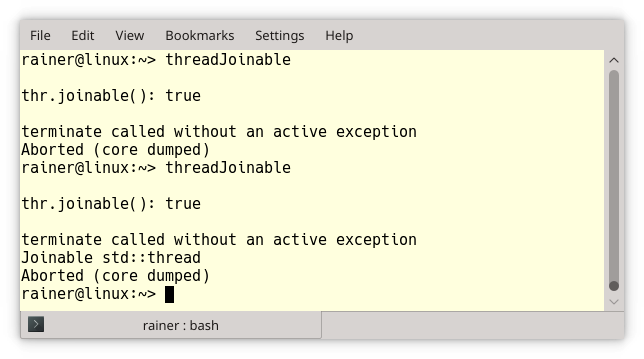
\includegraphics[width=0.8\textwidth]{content/2/chapter3/images/9.png}\\
对可汇入线程使用std::terminate
\end{center}

程序的两次执行都将终止。在第二次运行中,线程thr有足够的时间显示它的消息:" Joinable std::thread "。

修改后的示例中,我使用了C++20标准的std::jthread。

\hspace*{\fill} \\ %插入空行
\noindent
\textbf{线程thr会自动汇入}
\begin{lstlisting}[style=styleCXX]
int main() {
	std::cout << '\n';
	
	std::cout << std::boolalpha;
	std::jthread thr{[]{ std::cout << "Joinable std::jthread" << '\n'; }};
	std::cout << "thr.joinable(): " << thr.joinable() << '\n';
	
	std::cout << '\n';
}
\end{lstlisting}

现在,线程thr可在析构函数中进行汇入。

\begin{center}
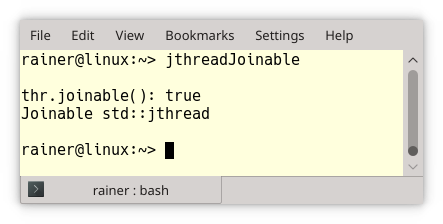
\includegraphics[width=0.6\textwidth]{content/2/chapter3/images/10.png}\\
线程thr自动汇入
\end{center}

\subsubsubsection{3.4.6\hspace{0.2cm}同步输出流}

C++20中,有了同步的输出流。当更多线程并发地写入std::cout,但没有同步时,会发生什么?

\hspace*{\fill} \\ %插入空行
\noindent
\textbf{未同步写入std::cout}
\begin{lstlisting}[style=styleCXX]
void sayHello(std::string name) {
	std::cout << "Hello from " << name << '\n';
}

int main() {
	std::cout << "\n";
	
	std::jthread t1(sayHello, "t1");
	std::jthread t2(sayHello, "t2");
	std::jthread t3(sayHello, "t3");
	std::jthread t4(sayHello, "t4");
	std::jthread t5(sayHello, "t5");
	std::jthread t6(sayHello, "t6");
	std::jthread t7(sayHello, "t7");
	std::jthread t8(sayHello, "t8");
	std::jthread t9(sayHello, "t9");
	std::jthread t10(sayHello, "t10");
	
	std::cout << '\n';
}
\end{lstlisting}

输出可能会弄得一团糟。

\begin{center}
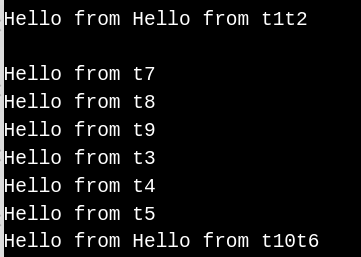
\includegraphics[width=0.6\textwidth]{content/2/chapter3/images/11.png}\\
未同步写入std::cout
\end{center}

从函数sayHello中的std::cout,切换到std::osyncstream(std::cout)可消除混乱。

\hspace*{\fill} \\ %插入空行
\noindent
\textbf{同步写入std::cout}
\begin{lstlisting}[style=styleCXX]
void sayHello(std::string name) {
	std::osyncstream(std::cout) << "Hello from " << name << '\n';
}
\end{lstlisting}

\begin{center}
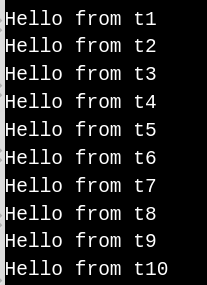
\includegraphics[width=0.4\textwidth]{content/2/chapter3/images/12.png}\\
同步写入std::cout
\end{center}
